\section{Vom Bild zum Vektor} \label{sec:vectormatrix}
\begin{tcolorbox}
	\centerline{\textbf{Lernziele Kapitel~\ref{sec:vectormatrix}}}
	\begin{enumerate}[leftmargin=*,label=\thesection.\arabic*]
		\item \label{item:vectormatrix_theory} Die Lernenden können für niedrige Auflösung ($M\cdot N<10$) die Umrechnungen zwischen Bild, Matrix und Vektor von Hand ausführen.\\
		(Aufgabe~\ref{aufg:vectormatrix_theory} und~\ref{aufg:vectormatrix_theory_1})
		\item \label{item:vectormatrix_code} Die Lernenden können in Python die Einträge von Vektoren und Matrizen auslesen und verändern.\\
		(Aufgabe~\ref{aufg:vectormatrix_code} und~\ref{aufg:negative})
	\end{enumerate}
\end{tcolorbox}
Der erste Schritt besteht darin, Bilder als Vektoren aufzufassen.
Das hat zwei Gründe: Erstens können wir diese nur so geeignet in Python darstellen und manipulieren.
Zweitens erlaubt uns das, Bilder in den Kontext der linearen Algebra zu bringen um deren mächtige Methoden anzuwenden.
Als Beispiel betrachten wir ein Bild der Auflösung $M=180$ Pixel (Höhe) mal $N=144$ Pixel (Breite), wie in Abbildung~\ref{fig:image_to_vector}.
Jedem Pixel wird nun eine reelle Zahl zwischen 0 und 1 zugeordnet.
Dabei bedeutet 0, dass das Pixel schwarz ist und 1 bedeutet, dass es weiss ist.
Die reellen Zahlen dazwischen beschreiben die Graustufen.
Wir Nummerieren diese Pixel mit zwei Indices $\left(m,n\right)$, wobei $1\leq m\leq M$ und $1\leq n\leq N$.
Zum Beispiel entspricht $\left(1,N\right)$ dem Pixel in der oberen rechten Ecke des Bildes.
Diesem Pixel wird also eine Zahl $p_{mn}$ zugeordnet, wobei $0\leq p_{mn}\leq 1$.
Das gibt uns eine $M\times N$-Matrix deren Einträge gerade die $p_{mn}$ sind.
So können wir also ein schwarz-weiss Bild als Matrix auffassen.
Nun schreiben wir die Spalten dieser Matrix in einen Vektor wie in Abbildung~\ref{fig:image_to_vector} gezeigt.
Damit erhalten wir eine eindeutige Korrespondenz zwischen schwarz-weiss Bilder der Auflösung $M\times N$ und Vektoren der Länge $M\cdot N$ mit Einträgen zwischen 0 und 1.
Für diesen Schritt ist es egal ob das Bild ein Gesicht zeigt oder etwas anderes.
\begin{figure}[ht]
	\centering
	\begin{tabular}{m{3.5cm} m{1cm} c m{1cm} c}
		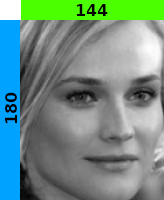
\includegraphics[width=0.2\textwidth]{images/vectormatrix/ImageToVector} &
		$\longleftrightarrow$ &
		$\begin{pmatrix}
			\textcolor{violet}{p_{11}} & \textcolor{orange}{p_{12}} & \cdots & \textcolor{olive}{p_{1N}} \\
			\textcolor{violet}{\vdots} & \textcolor{orange}{\vdots} & \ddots & \textcolor{olive}{\vdots} \\
			\textcolor{violet}{p_{M1}} & \textcolor{orange}{p_{M2}} & \cdots &  \textcolor{olive}{p_{MN}} \\
		\end{pmatrix}$ &
		$\longleftrightarrow$ &
		$\begin{pmatrix}
			\textcolor{violet}{p_{11}} \\
			\textcolor{violet}{\vdots} \\
			\textcolor{violet}{p_{M1}} \\
			\textcolor{orange}{p_{12}} \\
			\textcolor{orange}{\vdots} \\
			\textcolor{orange}{p_{M2}} \\
			\vdots \\
			\textcolor{olive}{p_{1N}} \\
			\textcolor{olive}{\vdots} \\
			\textcolor{olive}{p_{MN}} \\
		\end{pmatrix}$
	\end{tabular}
	\caption{Ein schwarz-weiss Bild kann als Matrix oder Vektor aufgefasst werden.}
	\label{fig:image_to_vector}
\end{figure}
\begin{aufgabe} \label{aufg:vectormatrix_theory}
	Man betrachte das schwarz-weiss Bild, welches durch folgende Matrix beschrieben ist.
	\begin{equation*}
		\begin{pmatrix}
			1 & \frac{1}{4} \\
			\frac{1}{2} & 0 \\
			0 & \frac{3}{4} \\
		\end{pmatrix}
	\end{equation*}
	\begin{enumerate}[label=(\alph*)]
		\item Welche Werte für $M$ und $N$ beschreiben die Auflösung dieses Bildes?
		\item Wie sieht der Vektor aus, der dieses Bild beschreibt?
		\item \label{item:image3x2} Welches der folgenden drei Bilder entspricht dieser Matrix?
		
		\definecolor{onefourth}{rgb}{0.25, 0.25, 0.25}
		\definecolor{onehalf}{rgb}{0.5, 0.5, 0.5}
		\definecolor{threefourth}{rgb}{0.75, 0.75, 0.75}
		
		\qquad\qquad
		
\begin{tikzpicture}
			\draw[step=1cm,white,very thin] (0,0) grid (2,3);
			\fill[white] (0,0) rectangle (1,1);
			\fill[onefourth] (1,0) rectangle (2,1);
			\fill[onehalf] (0,1) rectangle (1,2);
			\fill[white] (1,1) rectangle (2,2);
			\fill[black] (0,2) rectangle (1,3);
			\fill[threefourth] (1,2) rectangle (2,3);
		\end{tikzpicture}
		\qquad\qquad
		
\begin{tikzpicture}
			\draw[step=1cm,white,very thin] (0,0) grid (2,3);
			\fill[black] (0,0) rectangle (1,1);
			\fill[threefourth] (1,0) rectangle (2,1);
			\fill[onehalf] (0,1) rectangle (1,2);
			\fill[black] (1,1) rectangle (2,2);
			\fill[white] (0,2) rectangle (1,3);
			\fill[onefourth] (1,2) rectangle (2,3);
		\end{tikzpicture}
		\qquad\qquad
		
\begin{tikzpicture}
			\draw[step=1cm,white,very thin] (0,0) grid (2,3);
			\fill[black] (0,0) rectangle (1,1);
			\fill[onefourth] (1,0) rectangle (2,1);
			\fill[onehalf] (0,1) rectangle (1,2);
			\fill[black] (1,1) rectangle (2,2);
			\fill[white] (0,2) rectangle (1,3);
			\fill[threefourth] (1,2) rectangle (2,3);
		\end{tikzpicture}
	\end{enumerate}
\end{aufgabe}
\begin{losung}
	Die Lösung der ersten beiden Teilaufgaben kann von Abbildung~\ref{fig:image_to_vector} abgelesen werden.
	Für die letzte Teilaufgabe erinnern wir uns, dass die Zahlen zwischen 0 und 1 fliessend den Graustufen von Schwarz (Null) bis Weiss (Eins) entsprechen.
	\begin{enumerate}[label=(\alph*)]
		\item Die Auflösung ist $M=3$ mal $N=2$ Pixel.
		\item Der Vektor ist gegeben durch
		\begin{equation*}
			\begin{pmatrix}
				1 \\ \frac{1}{2} \\ 0 \\ \frac{1}{4} \\ 0 \\ \frac{3}{4} \\
			\end{pmatrix}.
		\end{equation*}
		\item Das mittlere Bild entspricht der Matrix.
	\end{enumerate}
\end{losung}
\begin{aufgabe} \label{aufg:vectormatrix_theory_1}
	Man betrachte den Vektor
	\begin{equation*}
		\begin{pmatrix}
			\frac{3}{4} \\ 0 \\ \frac{1}{4} \\ 0 \\ \frac{1}{2} \\ 1
		\end{pmatrix}.
	\end{equation*}
	Dieser soll ein Bild der Auflösung $M=2$ und $N=3$ beschreiben.
	\begin{enumerate}[label=(\alph*)]
		\item Schreiben Sie die entsprechende Matrix gemäss Abbildung~\ref{fig:image_to_vector} auf.
		\item Zeichnen Sie das entsprechende schwarz-weiss Bild, analog zu Teil~\ref{item:image3x2} in Aufgabe~\ref{aufg:vectormatrix_theory}.
	\end{enumerate}
\end{aufgabe}
\begin{losung}
	\begin{enumerate}[label=(\alph*)]
		\item Die Matrix hat nun $M=2$ Zeilen und $N=3$ Spalten. Nach Abbildung~\ref{fig:image_to_vector} erhalten wir
		\begin{equation*}
			\begin{pmatrix}
				\frac{3}{4} & 0 & \frac{1}{4} \\
				0 & \frac{1}{2} & 1
			\end{pmatrix}.
		\end{equation*}
		\item Das entsprechende schwarz-weiss Bild lässt sich von obiger Matrix ablesen:
		
		\definecolor{onefourth}{rgb}{0.25, 0.25, 0.25}
		\definecolor{onehalf}{rgb}{0.5, 0.5, 0.5}
		\definecolor{threefourth}{rgb}{0.75, 0.75, 0.75}
		\begin{center}
		
\begin{tikzpicture}
			\draw[step=1cm,white,very thin] (0,0) grid (3,2);
			\fill[white] (0,0) rectangle (1,1);
			\fill[onehalf] (1,0) rectangle (2,1);
			\fill[black] (2,0) rectangle (3,1);
			\fill[onefourth] (0,1) rectangle (1,2);
			\fill[white] (1,1) rectangle (2,2);
			\fill[threefourth] (2,1) rectangle (3,2);
		\end{tikzpicture}
		\end{center}

		Natürlich können Sie nicht die exakten Graustufen wiedergeben.
		Aber ihr Bild sollte vier verschiedene Graustufen enthalten, die richtig auf die Pixel verteilt sind.
	\end{enumerate}
\end{losung}
In unserem Python Code ist die Funktion, welche eine $M\times N$ Matrix auf diese Weise in einen Vektor der Länge $M\cdot N$ überführt, bereits implementiert.
Sie befindet sich im File \texttt{chapter2.py} und heisst \texttt{matrix\_to\_vector}.
Wir betrachten diese nun etwas genauer, um die Manipulation von Matrizen und Vektoren in Python zu lernen.
\lstinputlisting[firstline=12,lastline=17,style=python]{solution/chapter2.py}
Das Argument \texttt{P} ist eine \texttt{M} mal \texttt{N} Matrix und besteht aus den Einträgen $p_{mn}$ wie oben.
Auf die Einträge von Vektoren und Matrizen kann über die eckigen Klammern $[\ldots]$ zugegriffen werden.
Wir brauchen aber auch die Umkehrung dieser Operation.
Das ist der Zweck folgender Übung.
\begin{aufgabe} \label{aufg:vectormatrix_code}
	Ergänzen Sie im File \texttt{chapter2.py} die Funktion \texttt{vector\_to\_matrix(v, M, N)}.
	Dabei ist \texttt{v} ein Vektor der Länge $\texttt{M}\cdot\texttt{N}$ wie oben.
	Die Funktion soll die zu \texttt{v} gehörende Matrix zurück geben.
	Sie können die ihre Lösung überprüfen indem Sie das Skript \texttt{chapter2.py} laufen lassen.
\end{aufgabe}
\begin{losung}
	Bei einer richtigen Lösung sollte das Skript \texttt{chapter2.py} das Foto aus Abbildung~\ref{fig:image_to_vector} generieren.
	Die Lösung könnte zum Beispiel so aussehen:
\lstinputlisting[firstline=4,lastline=9,style=python]{solution/chapter2.py}
\end{losung}
Man kann gewisse Effekte in einem Bild erzeugen, indem man den zugehörigen Vektor manipuliert und anschliessend wieder als Bild darstellt.
Zum Beispiel kann man das Negativ eines gegebenen schwarz-weiss Bildes generieren.
Dazu nimmt man den Vektor $\vec p$ der Länge $M\cdot N$, welcher dieses Bild darstellt, und definiert damit einen neuen Vektor wie folgt
\begin{equation*}
	\vec p=
	\begin{pmatrix}
		p_1 \\ p_2 \\ \vdots \\ p_{M\cdot N} \\
	\end{pmatrix}
	\quad\longrightarrow\quad
	\begin{pmatrix}
		1-p_1 \\ 1-p_2 \\ \vdots \\ 1-p_{M\cdot N} \\
	\end{pmatrix}.
\end{equation*}
Der Vektor auf der rechten Seite entspricht dem Negativ des ursprünglichen Bildes.
Wie dieses Bild genau aussieht, sehen wir in der nächsten Aufgabe.
\begin{aufgabe} \label{aufg:negative}
	Ergänzen Sie im Skript \texttt{chapter2.py} die Funktion \texttt{get\_negative.py}.
	Diese soll zu einem gegeben Vektor \texttt{p} mit Einträgen zwischen 0 und 1 den Vektor des entsprechenden Negativs zurückgeben, wie oben beschrieben.
	Lassen Sie das Skript \texttt{chapter2.py} laufen um das entsprechende Bild auszugeben und um Ihre Lösung zu überprüfen.
\end{aufgabe}
\begin{losung}
	Links ist eine mögliche Implementierung gezeigt.
	Rechts ist ein Bild und dessen Negativ.\\[0.5cm]
	\begin{minipage}{0.45\textwidth}
\lstinputlisting[firstline=19,lastline=23,style=python]{solution/chapter2.py}
	\end{minipage}\hfill
	\begin{minipage}{0.25\textwidth}\vspace{-1cm}
		\centering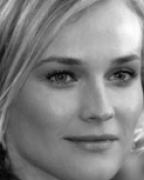
\includegraphics[width=0.6\textwidth]{images/vectormatrix/Diane_Kruger}
	\end{minipage}
	\begin{minipage}{0.25\textwidth}\vspace{-1cm}
		\centering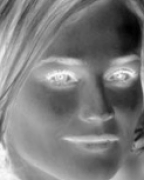
\includegraphics[width=0.6\textwidth]{images/vectormatrix/Diane_Kruger_negative}
	\end{minipage}
\end{losung}